\begin{enumerate}[label=\thesubsection.\arabic*.,ref=\thesubsection.\theenumi]
\numberwithin{equation}{enumi}
\item Using Nyquist criterion, find out whether the system below is stable or not.
\begin{align}
\label{eq:ee18btech11011_system}
 G(s)=\frac{20}{s(s+1)} , 
 H(s)=\frac{s+3}{s+4}
\end{align}
\solution The following python code generates the Nyquist plot in Fig.\ref{fig:ee18btech11011}.
\begin{lstlisting}
codes/ee18btech11011(1).ipynb
\end{lstlisting}
\begin{figure}[ht!]
  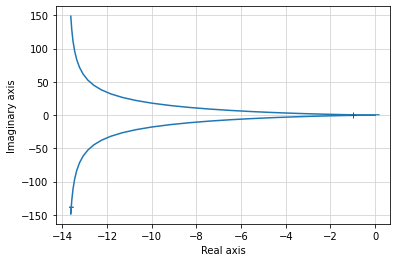
\includegraphics[width=\columnwidth]{ee18btech11011.png}
  \caption{Nyquist Plot}
  \label{fig:ee18btech11011}
\end{figure}
\begin{figure}[ht!]
  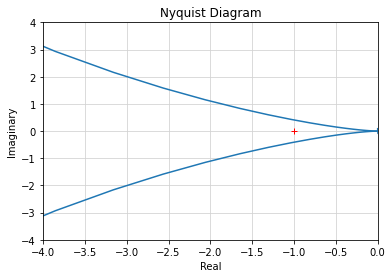
\includegraphics[width=\columnwidth]{zoomed.png}
  \caption{Zoomed image}
  \label{fig:zoomed}
\end{figure}
From Table \ref{table:EE18btech11007} we already know the Nyquist Stability criterion so for this closed loop system the transfer function will be =
\begin{align}
    \frac{G(s)}{1+G(s)H(s)}
\end{align}
\begin{align}
    \implies G(s)H(s)= \frac{20(s+3)}{s(s+1)(s+4)}
\end{align}
 So it has 3 open-loop poles 0,-1 and -4, therefore P=0.Further we know that N = Z-P , now we know Z = Poles of $\frac{G(s)}{1+G(s)H(s)}$in right half of s plane.To find the poles we can use the following Routh Hurwitz python code.Using this we get Z = 0.
 \begin{lstlisting}
codes/Routh.py
\end{lstlisting}
\begin{align}
    P = 0 , Z = 0
\end{align}
\begin{align}
    \implies N= 0
\end{align}
This can also be seen from the Fig. \ref{fig:ee18btech11011} that the encirclement is counter-clockwise not clockwise.Hence the system is stable.

\end{enumerate}

